%!TEX program = xelatex
\documentclass[a4paper,UTF8]{article}
\usepackage{ctex}
\usepackage[margin=1.25in]{geometry}
\usepackage{color}
\usepackage{graphicx}
\usepackage{amssymb}
\usepackage{amsmath}
\usepackage{amsthm}
\usepackage{enumerate}
\usepackage{bm}
\usepackage{hyperref}
\usepackage{epsfig}
\usepackage{color}
\usepackage{mdframed}
\usepackage{lipsum}
\usepackage{graphicx}
\usepackage{float}
\newmdtheoremenv{thm-box}{Theorem}
\newmdtheoremenv{prop-box}{Proposition}
\newmdtheoremenv{def-box}{定义}

\usepackage{listings}
\usepackage{xcolor}
\lstset{
	numbers=left,
	numberstyle= \tiny,
	keywordstyle= \color{ blue!70},
	commentstyle= \color{red!50!green!50!blue!50},
	frame=shadowbox, % 阴影效果
	rulesepcolor= \color{ red!20!green!20!blue!20} ,
	escapeinside=``, % 英文分号中可写入中文
	xleftmargin=2em,xrightmargin=2em, aboveskip=1em,
	framexleftmargin=2em
}

\usepackage{booktabs}

\setlength{\evensidemargin}{.25in}
\setlength{\textwidth}{6in}
\setlength{\topmargin}{-0.5in}
\setlength{\topmargin}{-0.5in}
% \setlength{\textheight}{9.5in}
%%%%%%%%%%%%%%%%%%此处用于设置页眉页脚%%%%%%%%%%%%%%%%%%
\usepackage{fancyhdr}
\usepackage{lastpage}
\usepackage{layout}
\footskip = 12pt
\pagestyle{fancy}                    % 设置页眉
\lhead{2021年春季}
\chead{模式识别}
% \rhead{第\thepage/\pageref{LastPage}页}
\rhead{作业一}
\cfoot{\thepage}
\renewcommand{\headrulewidth}{1pt}  			%页眉线宽,设为0可以去页眉线
\setlength{\skip\footins}{0.5cm}    			%脚注与正文的距离
\renewcommand{\footrulewidth}{0pt}  			%页脚线宽,设为0可以去页脚线

\makeatletter 									%设置双线页眉
\def\headrule{{\if@fancyplain\let\headrulewidth\plainheadrulewidth\fi%
\hrule\@height 1.0pt \@width\headwidth\vskip1pt	%上面线为1pt粗
\hrule\@height 0.5pt\@width\headwidth  			%下面0.5pt粗
\vskip-2\headrulewidth\vskip-1pt}      			%两条线的距离1pt
 \vspace{6mm}}     								%双线与下面正文之间的垂直间距
\makeatother

%%%%%%%%%%%%%%%%%%%%%%%%%%%%%%%%%%%%%%%%%%%%%%
\numberwithin{equation}{section}
%\usepackage[thmmarks, amsmath, thref]{ntheorem}
\newtheorem{theorem}{Theorem}
\newtheorem*{definition}{Definition}
\newtheorem*{solution}{Solution}
\newtheorem*{prove}{Proof}
\newcommand{\indep}{\rotatebox[origin=c]{90}{$\models$}}

\usepackage{multirow}

%--

%--
\begin{document}
\title{模式识别\\
作业一}
\author{181220076, 周韧哲, 本科,人工智能学院,人工智能学院选课}
\maketitle

\section*{Problem 1}
\begin{enumerate}[(a)]
	\item 需要令$\frac{8a-1}{3}\geq 0$,即$a\geq\frac{1}{8}$。
	\item 等于$1$。
	\item 当$a=\frac{1}{2}$,上式为$1$。我认为上式恒等于$1$。
	\item 返回值为$1.2182 + 0.1260i$。
	\item 原因是使用\^(1/3)命令时会调用pow(A,B),当B的绝对值(这里是$\frac{1}{3}$)小于1时会返回复数根。使用nthroot(A,B)命令可以得到正确结果为1。多个a的取值支持了我的想法。
	\item 证明:先令$x=\sqrt\frac{8a-1}{3}$,则$a=\frac{3x^2+1}{8}$,代入原式,得到
	      \begin{align*}
	      	&\quad\sqrt[3]{\frac{3x^2+1}{8}+\frac{\frac{3x^2+1}{8}+1}{3}}x+\sqrt[3]{\frac{3x^2+1}{8}-\frac{\frac{3x^2+1}{8}+1}{3}}x\\
	      	&=\sqrt[3]{\frac{1}{8}(x^3+3x^2+3x+1)}+\sqrt[3]{\frac{1}{8}(-x^3+3x^2-3x+1)}\\
	      	&=\sqrt[3]{\frac{1}{8}(x+1)^3}+\sqrt[3]{\frac{1}{8}(1-x)^3}\\
	      	&=1
	      \end{align*}
	\item 当$a=2$时,此表达式刚好符合上述定理,所以等于$1$。
	\item 由Cardano's formula知当$4p^3+27q^2>0$时,此式有唯一实数根
	$$\sqrt[3]{-\frac{q}{2}+\sqrt{\frac{q^2}{4}+\frac{p^3}{27}}} +\sqrt[3]{-\frac{q}{2}-\sqrt{\frac{q^2}{4}+\frac{p^3}{27}}}$$
	当$p=2a-1,q=-2a$时,方程变为$z^3+(2a-1)z-2a=0$,容易看出其有唯一实数根$1$,且将$p,q$代入上面的实数根表达式后恰好得到本题关于$a$的表达式,所以本题中的表达式等于$1$。
	
\end{enumerate}

\section*{Problem 2}

\begin{enumerate}[(a)]
	\item $x_{\perp}=\frac{x^Ty}{y^Ty}y=\frac{2\sqrt{3}}{4}\cdot(1,\sqrt{3})^T=(\frac{\sqrt{3}}{2},\frac{3}{2})^T$。
	\item $x-x_{\perp}=(\frac{\sqrt{3}}{2},-\frac{1}{2})^T$,所以$(x-x_{\perp})^Ty=\frac{\sqrt{3}}{2}-\frac{\sqrt{3}}{2}=0$,所以$y\perp (x-x_{\perp})$。
	\item \begin{figure}[b]
		\centering
		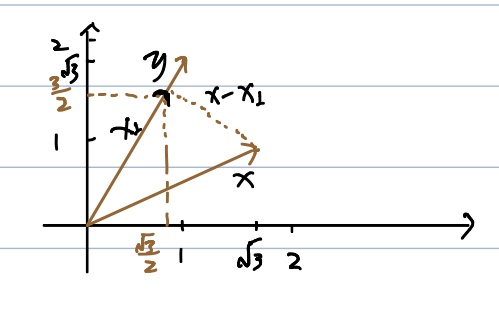
\includegraphics[width=0.3\textwidth]{1.jpg}
		\label{fig:1}
	\end{figure}
    如下图所示。
	\item 由提示得$\|x-x_{\perp}\|^2\leq \|x-\lambda y\|^2$,所以$\|x-x_{\perp}\|\leq \|x-\lambda y\|$,等号取得条件为$\|x_{\perp}-\lambda y\|=0$,即$\lambda=\frac{\sqrt{3}}{2}$。
\end{enumerate}


\section*{Problem 3}
\begin{enumerate}[(a)]
	\item 实对称矩阵正定的充要条件是特征值都是正数,所以$X$为正定矩阵的充要条件为$x>0$。
	\item $det(X)$等于$X$的特征值乘积,所以$12x=72$,$x=6$。
\end{enumerate}

\section*{Problem 4}
\begin{enumerate}[(a)]
	\item $\mathbb{E}[X]=\int_{-\infty}^{\infty}p(x)xdx=\int_{0}^{\infty}\beta e^{-\beta x }xdx=-\int_{0}^{\infty}xde^{-\beta x }=\int_{0}^{\infty}e^{-\beta x }dx-xe^{-\beta x }|_{0}^{\infty}=\frac{1}{\beta}$,\\
	$\mathbb{E}[X^2]=\int_{-\infty}^{\infty}p(x)x^2dx=-\int_{0}^{\infty}x^2de^{-\beta x }=2\int_{0}^{\infty}xe^{-\beta x }dx-x^2e^{-\beta x }|_{0}^{\infty}=\frac{2}{\beta^2}$,所以\\$Var(X)=\mathbb{E}[X^2]-(\mathbb{E}[X])^2=\frac{1}{\beta^2}$
	\item 易知$x<0$时,$F(x)=0$;当$x\geq0$时,$F(x)=\int_{0}^{x}p(t)dt=\int_{0}^{x}\beta e^{-\beta t}dt=1-e^{-\beta x}$
	\item 贝叶斯公式:$Pr(X\geq a+b| X\geq a)=\frac{Pr(X\geq a+b)}{Pr(X\geq a)}=\frac{1-F(a+b)}{1-F(a)}=e^{-\beta b}=1-F(b)=Pr(X\geq b)$
	\item 易得期望寿命为$\mathbb{E}[X]=\frac{1}{10^{-3}}=10^3$。由于指数分布的无记忆性,2000小时后的能再工作b小时的概率$Pr(X\geq b+2000|X\geq 2000)=Pr(X\geq b)$,故剩余寿命的期望不变,仍为$10^3$。
\end{enumerate}

\section*{Problem 5}
\begin{enumerate}[(a)]
	\item 因为$f''(x)=a^2e^{ax}\geq 0$,所以$f(x)$为凸函数。
	\item 因为$f''(x)=-\frac{1}{x^2}< 0$,所以$f(x)$为凹函数。
	\item $x>0$时,$f''(x)=\frac{1}{x}>0$,为凸函数。扩充定义域到$[0,\infty)$后,对于$0\leq\lambda\leq 1$,当$x=y=0$有$f(\lambda x+(1-\lambda)y)=0=\lambda f(x)+(1-\lambda)f(y)$成立;当其中一个不为0,不妨令$x=0$,则$f(\lambda x+(1-\lambda)y)=(1-\lambda) y\ln((1-\lambda)y)\leq (1-\lambda)y\ln y= \lambda f(x)+(1-\lambda)f(y)$,所以$f(x)$在$[0,\infty)$为凸函数。
	\item 约束为$g(p_1,\cdots,p_n)=\sum_{i=1}^{n}p_i=1$,令$f(p_1,\cdots,p_n)=-H=\sum_{i=1}^n p_i\log p_i$,则问题成为
	\begin{align*}
		&\min f(p_1,\cdots,p_n),\\&\text{ s.t. }g(p_1,\cdots,p_n)=1
	\end{align*}
    使用拉格朗日乘子法,拉格朗日函数$L(p_1,\cdots,p_n,\lambda)=f(p_1,\cdots,p_n)+\lambda(g(p_1,\cdots,p_n)-1)$,对各变量求导得
    \begin{align*}
    	&\frac{\partial L}{\partial p_i}=\log p_i+1+\lambda = 0,\quad i=1,\cdots,n\\
    	&\frac{\partial L}{\partial \lambda}=\sum_{i=1}^n p_i-1 = 0
    \end{align*}	
    解得$\lambda=\log n-1,\quad p_i=\frac{1}{n},i=1,\cdots,n$。所以最大化熵的$p_i$都相等且为$\frac{1}{n}$。
\end{enumerate}

\end{document}